\documentclass[12pt, titlepage]{article}

\usepackage{booktabs}
\usepackage{tabularx}
\usepackage{hyperref}
\hypersetup{
    colorlinks,
    citecolor=black,
    filecolor=cyan,
    linkcolor=red,
    urlcolor=blue
}
\usepackage[round]{natbib}
\usepackage{graphicx}
\graphicspath{ {img/} }

\title{SE 3XA3: Test Plan\\ReTouch}

\author{Team \#7, ReTouchers
		\\ Abrar Attia - attiaa1
		\\ Susan Fayez - fayezs
		\\ Mediha Munim - munimm
}

\date{\today}

\begin{document}

\maketitle

\pagenumbering{roman}
\tableofcontents
\listoftables
\listoffigures

\begin{table}[bp]
\caption{\bf Revision History}
\begin{tabularx}{\textwidth}{p{3cm}p{2cm}X}
\toprule {\bf Date} & {\bf Version} & {\bf Notes}\\
\midrule
Date 27 & 1.0 & PoC, and Unit Tests added\\
October 27 & 1.0 & Added general information\\
\bottomrule
\end{tabularx}
\end{table}

\newpage

\pagenumbering{arabic}

This document describes the test plan that shall be followed for ReTouch.

\section{General Information}

\subsection{Purpose}

	The purpose of this project is to re-implement the open source project K-Touch. K-Touch is a utility that allows users to track their speed and accuracy in typing, and results in improved typing skills through practice and repetition. The re-implementation will improve upon the original project by making it more user friendly and providing more comprehensive documentation. The purpose of this document is to make the testing for ReTouch as efficient as possible to ensure a robust, complete, and fully-functional program.

\subsection{Scope}

	The scope of ReTouch will be to improve KTouch by making it available on other operating systems while improving much of the functionality and user experience, while still providing an intuitive GUI and a user guide. Therefore, testing ReTouch will involve testing the GUI, the user input, file input and output, and the other algorithms. 

\subsection{Acronyms, Abbreviations, and Symbols}
	
\begin{table}[hbp]
\caption{\textbf{Table of Abbreviations}} \label{Table}

\begin{tabularx}{\textwidth}{p{3cm}X}
\toprule
\textbf{Abbreviation} & \textbf{Definition} \\
\midrule
GUI & Graphical User Interface\\
Abbreviation2 & Definition2\\
\bottomrule
\end{tabularx}

\end{table}

\begin{table}[!htbp]
\caption{\textbf{Table of Definitions}} \label{Table}

\begin{tabularx}{\textwidth}{p{3cm}X}
\toprule
\textbf{Term} & \textbf{Definition}\\
\midrule
Term1 & Definition1\\
Term2 & Definition2\\
\bottomrule
\end{tabularx}

\end{table}	

\subsection{Overview of Document}

	This document outlines several types of tests that the ReTouchers team plans to use, potential testing tools, a testing schedule, and specific test cases that will cover the functional and non-functional requirements of ReTouch. 

\section{Plan}
	
\subsection{Software Description}

\begin{figure}[h!]
	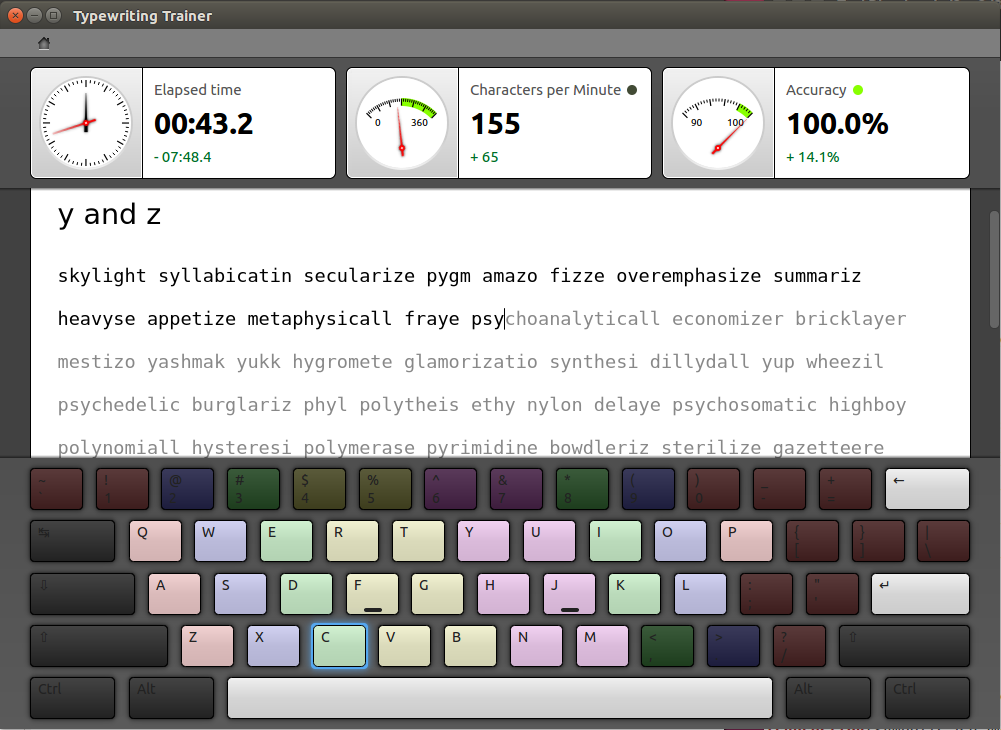
\includegraphics[scale=0.5]{KTouchLesson.png}
	\centering
	\caption{Visual Sample of K-Touch}
	\label{figure:1}
\end{figure}

	ReTouch will be implemented very similarly to K-Touch, the original application, in its functionality. The software shall begin by giving the user a list of lessons to choose from, where each lesson consists of a different combination of keyboard characters that the user can practice typing. The main program will begin at that point. A sequence of characters will appear on screen, and the user will be prompted to type those characters on the keyboard (as is seen in \hyperref[figure:1]{Figure 1}). The user must accurately type all of them (incorrectly typed characters can be erased and then typed again). The software will calculate the elapsed time, the user's typing accuracy, and the user's typing speed during the program's execution. Once the user has completed the lesson, the results of the lesson will appear on screen. The software will be implemented using Java.

\subsection{Test Team}

	The testing will be divided roughly equally among the ReTouchers team (Abrar Attia, Susan Fayez and Mediha Munim). Ideally, every member will be able to look over all of the components that need to be tested and contribute new cases to ensure robustness of the software, but this may not be possible due to the time constraints on the project. See the \hyperref[sec:ts]{Testing Schedule} for details.

\subsection{Testing Approach}

	Many different testing techniques will be utlized in the testing process. Black box testing will involve unit testing and integration testing. To automate these tests, the team will take advantage of JUnit's functionalities. Private methods will be tested as well, and ideally testing will take place throughout the implementation process to ensure that the tests that passed early on in the process will still pass after finalizing the code (regression testing). To test the internal framework of the software, white box testing will be used. Not all of the testing will be automatic - manual system testing will be vital to the final product because the project is expected to have a detailed GUI. Both static and dynamic test cases will be covered using tools described in \hyperref[sec:tt]{Testing Tools}. In system testing, the functionalities of KTouch can be compared to ReTouch to ensure that it works just as it was intended to by the original programmers. All in all, the ReTouchers team strives to test as efficiently and effectively as possible.

\subsection{Testing Tools}
\label{sec:tt}

	As mentioned earlier, the main tool for testing the Java code will be JUnit. Static testing can take place automatically as the project will be implemented in Eclipse, which has static testing capabilities. JaCoCo is a code coverage tool that works well with Eclipse. However, due to the time constraints associated with the project and the potential learning curve with the library, it may not be used. Finally, Apache JMeter will be used for load testing.

\subsection{Testing Schedule}
\label{sec:ts}
		
The Gantt Project, which illustrates the project schedule, can be found \href{run:../../ProjectSchedule/Gantt_Project.gan}{here} or in the ProjectSchedule directory. 

\section{System Test Description}
	
\subsection{Tests for Functional Requirements}

\subsubsection{Area of Testing1}
		
\paragraph{Title for Test}

\begin{enumerate}

\item{test-id1\\}

Type: Functional, Dynamic, Manual, Static etc.
					
Initial State: 
					
Input: 
					
Output: 
					
How test will be performed: 
					
\item{test-id2\\}

Type: Functional, Dynamic, Manual, Static etc.
					
Initial State: 
					
Input: 
					
Output: 
					
How test will be performed: 

\end{enumerate}

\subsubsection{Area of Testing2}

...

\subsection{Tests for Nonfunctional Requirements}

\subsubsection{Area of Testing1}
		
\paragraph{Title for Test}

\begin{enumerate}

\item{test-id1\\}

Type: 
					
Initial State: 
					
Input/Condition: 
					
Output/Result: 
					
How test will be performed: 
					
\item{test-id2\\}

Type: Functional, Dynamic, Manual, Static etc.
					
Initial State: 
					
Input: 
					
Output: 
					
How test will be performed: 

\end{enumerate}

\subsubsection{Area of Testing2}

...

\subsection{Traceability Between Test Cases and Requirements}

\section{Tests for Proof of Concept}

The Proof of Concept testing will focus on validating that all the identified risks in the development of the application can be overcome. The determined risks include running the code concurrently, such as running a constant timer alongside a main program that requests and waits for keyboard input. Another risk that needs to be resolved and tested includes 

\subsection{Area of Testing1}
		
\paragraph{Title for Test}

\begin{enumerate}

\item{test-id1\\}

Type: Functional, Dynamic, Manual, Static etc.
					
Initial State: 
					
Input: 
					
Output: 
					
How test will be performed: 
					
\item{test-id2\\}

Type: Functional, Dynamic, Manual, Static etc.
					
Initial State: 
					
Input: 
					
Output: 
					
How test will be performed: 

\end{enumerate}

\subsection{Area of Testing2}

...

	
\section{Comparison to Existing Implementation}	
There is currently no required tests to be done to compare the application to the existing implementation.
				
\section{Unit Testing Plan}

The JUnit unit testing framework will be used to implement the unit testing for the ReTouch application.
		
\subsection{Unit testing of internal functions}

When testing the internal functions of the application, the unit tests will be based on each methods input parameters and their expected versus derived outputs. Each method will be testing with standard expected inputs as well as exceptions to improve the programs robustness and reduce bugs. Additionally, every class in the program will include all the required import statements. Therefore, the unit tests will not require any stubs or drivers when testing individual methods or components that depend on multiple methods. 
		
\subsection{Unit testing of output files}

When testing the output files and program outputs, there will need to be a comparison between the required output and the generated output. However, at this time, there are no expected output files that will be created when the program is run. 		

\bibliographystyle{plainnat}

\bibliography{SRS}

\newpage

\subsection{Symbolic Parameters}

The definition of the test cases will call for SYMBOLIC\_CONSTANTS.
Their values are defined in this section for easy maintenance.

\subsection{Usability Survey Questions?}

This is a section that would be appropriate for some teams.

\end{document}
